\section{When later contracts cannot recover earlier meeting allocations}\label{sec:aggregation}
The calendar result identifies a limitation of the variance panel. We now give a stronger result for a particular contract family, allowing many strikes, later cash flows, and American cash exercise. In this section set $f_0=0$ and $\sigma=0$ in \eqref{eq:curve}. Use the usual augmentation of the filtration generated by the meeting surprises alone. These restrictions isolate the information lost when observation and exercise begin only after a group of meetings. This is a separate exact experiment, not the model used for the empirical calibration.

Fix a future cutoff $A\geq T_k$, with exactly $k$ meetings at or before $A$. These meetings are still future events from time zero. Write
\begin{equation}\label{eq:VH}
V=\sum_{i\leq k}v_i,\qquad M_1=\sum_{i\leq k}T_i v_i,\qquad y=r_A.
\end{equation}
Hold later meeting dates and variances fixed. For $t\geq A$ and $T\geq t$, direct substitution gives
\begin{equation}\label{eq:postcurve}
f(t,T)=y+V(T-A)+\sum_{A<T_i\leq t}\{X_i+v_i(T-T_i)\}.
\end{equation}
The curve after $A$ therefore remembers the earlier surprises through the single random level $y$ and the deterministic total $V$. It does not retain their individual variances.

\begin{theorem}[Aggregation after a cutoff]\label{thm:aggregate}
In this pure-jump model the following statements hold.
\begin{enumerate}
\item Under the probability measure with density $B_A^{-1}$ relative to $\Q$, $y$ has law $N(0,V)$ and is independent of all later surprises. The density has expectation one.
\item Consider a cash flow paid at $S\geq A$ that is a fixed Borel function of the curve history from $A$ to $S$, using the same function when the earlier variance allocation changes. If its discounted absolute value is integrable, its time-zero value depends on the earlier variances only through $V$.
\item Let $Y_t$, $A\leq t\leq S$, be an American cash payoff given by a fixed Borel, nonanticipating rule of the post-$A$ curve history, with the same rule across allocations. Suppose the payoff discounted back to $A$, $\widehat Y_t=(B_A/B_t)Y_t$, is adapted, has right-continuous paths with left limits, and satisfies $\sup_{A\leq t\leq S}|\widehat Y_t|\leq\mathcal M$ for an integrable $\mathcal M$ under the tilted measure. Then $\sup_\tau\E[B_\tau^{-1}Y_\tau]$, over full-history stopping times $\tau\in[A,S]$, depends on the earlier variances only through $V$.
\item For continuously compounded futures on windows $[a,b]$ with $a\geq A$,
\begin{equation}\label{eq:futureVH}
\log G_0(a,b)=\delta(bV-M_1)+\text{known later-meeting contribution}.
\end{equation}
Consequently allocations with the same $(V,M_1)$ give all the same values in this stated family. If the observations include two such futures with distinct terminal dates $b$, they determine $(V,M_1)$.
\end{enumerate}
\end{theorem}
The qualification that the payoff rule is the same is substantive. A claim that explicitly pays the unobserved parameter $v_1$, or a rule whose strike changes with $M_1$, is not a fixed contract in this family. The total $V$ may enter the payoff through the observed curve, including its slope; an allocation-dependent payoff rule is excluded. Ordinary fixed-strike cash claims on that curve satisfy the requirement.

The proof of the American statement does not assert that exercise is European or that early exercise has no value. It shows that the extra information about individual early surprises is independent randomization after the change of measure, and cannot improve the supremum over stopping rules. The path regularity and domination in part 3 permit approximation of continuous exercise by finite exercise grids; standard continuous-payoff cash options satisfy these sufficient conditions in this finite Gaussian model. Appendix~\ref{app:aggregation} gives the argument. Actual exchange delivery into futures positions is a separate contract convention.

The European result also covers products of bond-implied overnight accumulation factors after $A$. Define a fixing on $[u_j,u_{j+1}]$ by $L_j=(P(u_j,u_{j+1})^{-1}-1)/(u_{j+1}-u_j)$. Its product $\prod_j(1+(u_{j+1}-u_j)L_j)$ is a function of the post-$A$ curve. It equals $\exp(\int_a^b r_s\,\dd s)$ in this pure-jump model if no meeting lies strictly inside any fixing interval. Without that alignment the aggregation statement for the payoff still holds, but formula~\eqref{eq:futureVH} is not being asserted for the product. Bond-implied fixings are a model convention, not an identification with every realized SOFR fixing.

\subsection{The set of compatible allocations}
Given $(V,M_1)$, the possible early-meeting vectors are exactly
\begin{equation}\label{eq:polytope}
\Pi(V,M_1)=\left\{x\in\R_+^k:\ \sum_i x_i=V,\quad \sum_i T_i x_i=M_1\right\}.
\end{equation}
For $V\geq0$, this set is nonempty if and only if $T_1V\leq M_1\leq T_kV$. If $V=M_1=0$, it consists only of the zero vector. If $V>0$, it is compact. If it contains a strictly positive vector and $k\geq2$, its dimension is $k-2$: the two equality rows are independent because the meeting dates are distinct, and nonnegativity imposes no local restriction at that vector. Every coordinate reaches its minimum and maximum at an allocation with at most two positive coordinates. For a pair $i<j$, the candidate allocation is
\begin{equation}\label{eq:vertices}
x_i=\frac{T_jV-M_1}{T_j-T_i},\qquad
x_j=\frac{M_1-T_iV}{T_j-T_i},
\end{equation}
when both are nonnegative, with all other coordinates zero. A one-coordinate allocation is possible when $M_1=T_iV$. These candidates give sharp bounds by a finite calculation.

For three equally spaced meetings at $T_i=i/12$, $V=700$ bp$^2$, and $M_1=2V/12$, the set is
\[
(x_1,x_2,x_3)=(x,700-2x,x),\qquad 0\leq x\leq350.
\]
The two allocations in the introduction lie on this same line. The second meeting can have any variance between zero and $700$ bp$^2$, while preserving all observations in Theorem~\ref{thm:aggregate}. The bounds on different meetings are joint constraints: their coordinate intervals cannot be combined arbitrarily.

\begin{figure}[ht]
\centering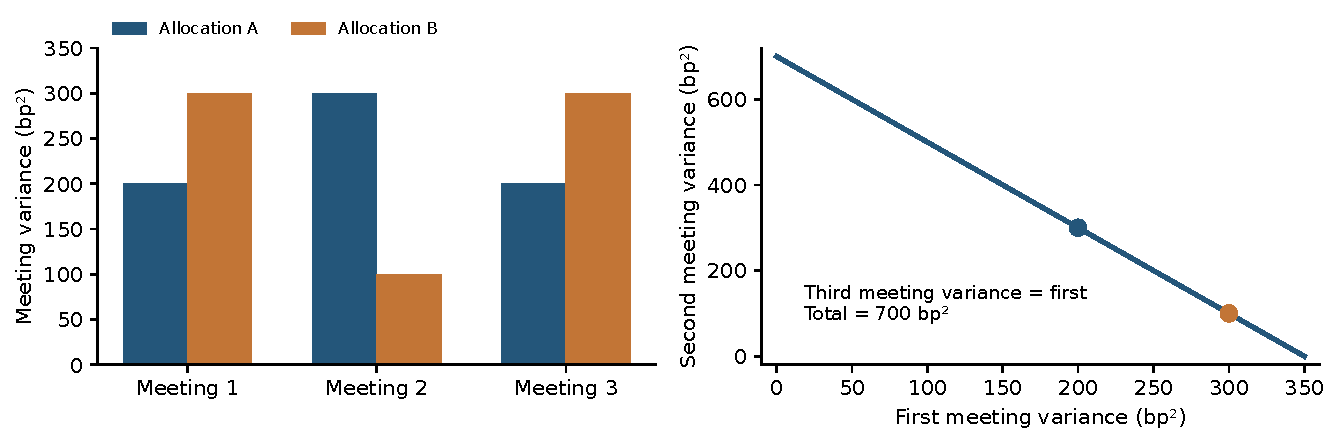
\includegraphics[width=.95\textwidth]{figures/aggregation.pdf}
\caption{Two different allocations with the same prices for the contract family in Theorem~\ref{thm:aggregate}. Left: the two allocations. Right: the entire compatible set for the first two coordinates; the third equals the first. The meeting dates are equally spaced.}\label{fig:aggregate}
\end{figure}

\subsection{A deterministic initial curve and continuous pre-cutoff risk}
The aggregation mechanism is not tied to a zero initial curve or to an absence of background volatility. The following extension connects it to the model of Section~\ref{sec:prices}. Keep the initial curve and all post-$A$ parameters fixed, and allow both the earlier meeting variances and the deterministic background volatility before $A$ to vary. Define
\begin{equation}\label{eq:generalaggregates}
V_A=\sum_{T_i\leq A}v_i+\int_0^A\sigma(s)^2\,\dd s,\qquad
M_{1,A}=\sum_{T_i\leq A}T_i v_i+\int_0^A s\sigma(s)^2\,\dd s.
\end{equation}
For this extension use the usual augmentation (completion and right-continuous regularization) of the natural filtration generated by
$Y_t=\int_0^t\sigma(s)\,\dd W_s$ and the meeting surprises revealed by time $t$. Thus exercise uses the history of the model's driving risks. The statement below does not allow an arbitrary larger filtration.

\begin{corollary}[Aggregation including continuous risk]\label{cor:generalaggregate}
For the model \eqref{eq:curve}, under the probability measure with density
$B_A^{-1}/P(0,A)$, the centred level $y_A=r_A-f_0(A)$ is $N(0,V_A)$ and independent of future driving increments. Fixed post-$A$ cash claims depend on the pre-$A$ variance allocation only through $V_A$, including American claims under the regularity and domination assumptions of Theorem~\ref{thm:aggregate}. For $a\geq A$,
\[
\log G_0(a,b)=\int_a^b f_0(x)\,\dd x+\delta(bV_A-M_{1,A})
                   +\text{fixed post-$A$ contribution}.
\]
Thus equal $(V_A,M_{1,A})$ gives equal prices for the same post-cutoff contract family.
\end{corollary}
\begin{proof}
Write $L_A=\int_0^A\sigma\,\dd W+\sum_{T_i\leq A}X_i$. Then
$y_A=L_A+AV_A-M_{1,A}$, and the normalized discount density is the Gaussian exponential with random exponent
\[
-\int_0^A(A-s)\sigma(s)\,\dd W_s-\sum_{T_i\leq A}(A-T_i)X_i.
\]
Its covariance with $L_A$ is $-(AV_A-M_{1,A})$. Exponential tilting therefore centres $y_A$ and preserves its variance $V_A$. For $t\geq A$,
\begin{align*}
f(t,T)={}&f_0(T)+y_A+V_A(T-A)+\int_A^t\sigma(s)\,\dd W_s\\
&+\int_A^t\sigma(s)^2(T-s)\,\dd s
  +\sum_{A<T_i\leq t}\{X_i+v_i(T-T_i)\}.
\end{align*}
For a nonnegative Borel cash payoff, integration against this state law gives a value depending on the earlier allocation only through $V_A$, multiplied by the fixed factor $P(0,A)$. An absolutely integrable signed payoff is the difference of its positive and negative parts, so the same conclusion follows by applying the nonnegative result twice.

For American exercise, when $V_A>0$, regress the early Gaussian history onto $y_A$ under the tilted measure. The centred residual history is independent of $y_A$ and of all future driving increments. Continuity of $Y$ allows its history to be recovered from rational-time coordinates, together with the finitely many revealed surprises. At each time $s\geq A$, the completed natural information therefore equals that generated by the residual history, $y_A$, and the driving increments from $A$ to $s$, with the same null sets adjoined. The strictly positive discount density preserves those null sets. Take right-continuous regularizations on both sides to obtain the exercise filtration.

Section a finite-grid stopping rule at each fixed residual history. Independence bounds its expectation by the supremum over rules using only $y_A$ and the future driving increments; those rules also give the reverse inequality. Upward grid approximation, right-continuity, and dominated convergence under the assumed integrable envelope extend the equality to continuous exercise. The envelope can be taken as the supremum of the discounted payoff over rational times and the terminal time, a Borel function of the post-cutoff state history. Consequently the value depends only on that history's law and $V_A$. When $V_A=0$, $y_A$ is deterministic and the same sectioning argument applies to the independent residual history. Finally $h(s)=\delta(b-s)$ before $A\leq a$ in \eqref{eq:p}, proving the futures identity.
\end{proof}
When pre-cutoff background variance is fixed, subtract its known total and first moment to recover the meeting-allocation polytope \eqref{eq:polytope}. When it is also unknown, the indistinguishable set includes both meeting allocations and continuous variance profiles with the same two moments. Later cash contracts cannot separate those components.

\subsection{Exercise convention changes value, but need not restore identification}
The pure-jump model gives an explicit cash-exercise formula after the last meeting. Let $T_N\leq A<S\leq a<b$, $\bar t=(a+b)/2$, and $L=S-A$. The futures rate is already known at $A$ and remains constant thereafter:
\[
F_t=\frac{\exp\{\delta r_A+\delta V(\bar t-A)\}-1}{\delta},
\qquad A\leq t\leq b.
\]
For $V>0$, define
\[
\mathcal D_{V,L}(x)=\max_{0\leq u\leq L}e^{-xu-Vu^2/2},\qquad
u_*(x)=\min\{L,\max\{0,-x/V\}\}.
\]
A call with rate strike $k$ and cash paid on exercise has value
\begin{equation}\label{eq:latecash}
U=\E_{Y\sim N(0,V)}
 \left[\left(\frac{e^{\delta Y+\delta V(\bar t-A)}-1}{\delta}-k\right)^+
                         \mathcal D_{V,L}(Y)\right].
\end{equation}
Indeed, $B_{A+u}/B_A=e^{r_Au+Vu^2/2}$; the known nonnegative payoff is maximized after discounting by exercise at $A+u_*(r_A)$. Tilting to $A$ gives \eqref{eq:latecash}. For every finite strike and $V>0$, cash exercise strictly improves on mandatory exercise at $S$: on a sufficiently large positive-$r_A$ set the call pays and immediate exercise discounts less. Yet its value still contains no information about individual earlier variances beyond $V$.

For comparison, define the futures-style exercise functional
\[
\widetilde U=\sup_{\tau\in\mathcal T[A,S]}\E[(F_\tau-k)^+],
\]
without cash discounting. Since $F$ is a martingale and the payoff is convex, conditional Jensen and optional sampling give
\begin{equation}\label{eq:futuresstyle}
\widetilde U=\E[(F_S-k)^+]
 =\frac1\delta\mathcal B\left(G_0,1+\delta k,
                         \sum_{T_i\leq S}w(T_i)^2v_i\right)
\end{equation}
for $1+\delta k>0$, with the intrinsic linear formula otherwise. This holds even when exercise spans unrevealed meetings; Gaussian exponential moments supply the required integrability. The no-early-exercise conclusion is the established result of \citet{lieu1990option,chen1993pricing}. Its identification consequence here is that earlier variances still enter only through $(V,M_1)$ when accrual starts after the cutoff. Additional expiries can identify later meetings with nonzero $w(T_i)$, but cannot resolve the earlier polytope.

The two formulas distinguish cash timing value from information about the earlier allocation. They do not identify the undiscounted functional with CME's premium-paid option convention. Exact cash exercise across one unrevealed meeting is given in Appendix~\ref{app:crossmeeting}; it depends on the earlier total and the crossed meeting variance separately.
